% To be used for generating only 1 chapter of the thesis

\title{Side-Channel Security in Networks: From the Internet to Interconnects}

\author{Rut Vora}
\previousdegree{B. Engineering in Computer Science, BITS-Pilani, 2020}


\degreetitle{Master of Science}

\institution{The University of British Columbia}
\campus{Vancouver}

\faculty{The Faculty of Graduate and Postdoctoral Studies}
\department{Computer Science}
\submissionmonth{March}
\submissionyear{2025}

\examiningcommittee{Aastha Mehta, Assistant Professor, Computer Science, \textsc{UBC}}{Supervisor}
% \examiningcommittee{Mathias L\'{e}cuyer, Assistant Professor, Computer Science, \textsc{UBC}}{Co-Supervisor}
% \examiningcommittee{Margo Seltzer, Professor, Computer Science, \textsc{UBC}}{Supervisory Committee Member}

%% hyperref package provides support for embedding meta-data in .PDF
%% files
\hypersetup{
  pdftitle={Side-Channel Security in Networks: From the Internet to Interconnects  (DRAFT: \today)},
  pdfauthor={Rut Vora},
  pdfkeywords={PCIe, CXL, Side Channels, Networks, Proxy}
}

\begin{document}

\maketitle

\textspacing		% begin one-half or double spacing

% Body of Thesis (not all sections may apply)
\mainmatter

\acresetall	% reset all acronyms used so far

% Main Sections
% \chapter{Background}

% We begin this chapter by discussing the problem of network side-channel attacks in \Cref{sec:ns-attacks}, in the context of two distinct applications: video streaming and web services.
% In \Cref{sec:dp-background}, we present a comprehensive definition of differential privacy (DP), outline its key properties, and highlight its primary applications, thereby setting the foundation for our differentially private traffic shaping mechanism.
% In \Cref{sec:background-quic} we provide a brief overview of the QUIC protocol, which plays a pivotal role in the design of {\sys}.
% Finally, in \Cref{sec:threat-model}, we conclude this chapter by explaining our threat model. 

\section{Network Side Channels}
\label{sec:network-side-channel-background}

Let us first understand how network side-channel attacks are carried out.
The ultimate goal of the attacker is to determine the contents of the web traffic being transmitted or received by the victim. More often than not, an attacker is interested in knowing if the victim accessed any content from a small subset and, if so, which content they accessed.
To do this, the attacker takes the following steps: 
1) Collect network traces
2) Build a classifier trained on the collected network traces
3) Gain access to the network shared with the victim
4) Profile the victim's network traffic
5) Determine whether the victim accessed any content of interest to the attacker

First, the attacker builds a collection of the content (e.g. webpages and video streams) that they are interested in. 
They collect network traces for this content under various network conditions to account for variability caused by the network itself. 
Then, the attacker trains a classifier on this collected network trace.
The classifier can use multiple features like packer sizes, inter-packer timing, total bytes transferred in a burst of packets, the duration of the burst and the interval between bursts, and the direction of the bursts \cite{schuster2017beautyburst}.

Next, the attacker infiltrates a machine that shares some network path with the victim.
This machine could also be the victim's machine. 
The malicious application could be a javascript-based advertisement on the page the victim is visiting or another process on the victim's machine, thus sharing the network card on that machine. 
It could also be a shared router/switch in the victim's network path to the server.
The attacker could either be another client connected to the same shared router/switch or someone who owns the router/switch.
If the attacker owns an element in the network path, they can directly observe all the features necessary to carry out the attack. 
Otherwise, they create congestion in the shared network path such that the victim's network traffic would contend with the attacker's traffic.
In this case, the attacker's traffic would be delayed, and the delay would be proportional to the victim's traffic, thus revealing some features of the victim's traffic.

The attacker collects the network traces of its own traffic and, based on that, extracts the features of the victim's traffic flow. These extracted features are then run through the pre-trained classifier, which helps the attacker determine which content the victim accessed. \citeauthor{schuster2017beautyburst} demonstrated that one could train a Convolution Neural Network (CNN)-based classifier to determine which video the victim is streaming. Similarly, prior work has demonstrated that such a network side channel-based approach can also be used to determine which webpage the victim is visiting \cite{hayes2016kfp, panchenko2016website, gong2010fingerprinting}

% \section{Threat Model}\label{sec:nsc-threat-model}

\section{NetShaper - Framework}
\label{sec:netshaper-framework-bg}

NetShaper \cite{sabzi2024netshaper} is both the name of a differential-privacy-based framework for mitigating network side-channel attacks and the system that utilises that framework. 
Here, we provide a brief description of the NetShaper Framework.

\subsection{Differential Privacy}
NetShaper's framework relies on Differential Privacy (DP) to provide robust, mathematical guarantees against side-channel attacks in internet networks.
DP is a framework originally proposed by \citeauthor{dwork2006differential} for releasing usable aggregate metrics regarding a dataset while limiting the leakage of information about individual data points in that dataset.
In other words, DP bounds the probability of an observer being able to infer if an individual data point was used to generate the aggregate metric the observer has access to.
DP has two main parameters: \\
\textbf{$\epsilon$: } Intuitively, it specifies the amount of privacy loss
\textbf{$\delta$: } Intuitively, it specifies the probability with which a given differentially-private mechanism can fail.


\begin{definition}[Differential privacy]
  \label{def:dp}
  A randomized algorithm $A_{DP}$ is $(\varepsilon, \delta)-DP$ if for all ${S} \subseteq Range(A_{DP})$ and for all datasets $D, D'$ that differ on a single element, we have:
  \begin{equation*}
    \Pr[A_{DP}(D) \in S] \leq \exp(\varepsilon)\Pr[A{DP}(D') \in S] + \delta
  \end{equation*}
\end{definition}

For any aggregate algorithm $A$, we can make an $(\varepsilon, \delta)-DP$ algorithm by adding some noise to the output of $A$.
There are many different mechanisms to add the noise $\eta$, but most commonly, $\eta$ is a function of $\varepsilon, \delta$ and other dataset-dependent parameters. 
Mathematically, $A_{DP}(D) = A(D) + \eta(\varepsilon, \delta, ...)$

DP has a few useful properties: 
\textbf{1) Post Processing:} Any further operations or processing on the output of an $(\varepsilon, \delta)-DP$ algorithm is also $(\varepsilon, \delta)-DP$.
This condition holds true as long as the operations carried out do not involve any auxiliary knowledge of the dataset.
\textbf{2) Composition:} It is possible to quantify the total privacy loss when multiple queries are issued to the same $(\varepsilon, \delta)-DP$ algorithm.

\subsection{Applying DP on network streams}
NetShaper uses DP to mitigate network side-channel attacks. 
To achieve this, NetShaper relies on two key ideas: 
First, NetShaper represents network traffic streams as datasets to which DP can be applied.
As DP applies to datasets, we must first represent a network stream as a dataset.
A network stream $S$ can be represented as a sequence of packets $P_i^S$, where each packet is associated with its length and the timestamp at which it was encountered (i.e. $P_i^S = (l_i^S, t_i^S$).
Hence, $S$ is the dataset consisting of the traffic shape, which can be used by an attacker to carry out a side-channel attack, as outlined in \Cref{sec:network-side-channel-background}.
As the network stream can potentially be long, NetShaper models the DP guarantees in windows of fixed length $W$ and can use composition to calculate the privacy loss across multiple windows.
Second, NetShaper relies on a buffering queue to control the shape of the traffic visible to the attacker within each window $W$ by discretising time into $W$-sized windows.
At the beginning of each discrete window, NetShaper checks the size of the buffer and adds DP noise to the size to determine the amount of data to be sent out in that window.


So, initially, the attacker was able to query a function $f(S, t_{start}, t_{end})$ to obtain the size and time of the packet that was transmitted by the victim. 
However, with the application of DP on the network stream, the attacker can now only query a new function $f_{DP}(S, t_{start}, t_{end})$.
$f_{DP}$ is a differentially private function ensuring that the probability of leaking individual entries of the dataset is bounded, and where $t_{end} - t_{start} = kW, k \in N$.

\endinput

Note: Should we add stuff about sensitivity? (I don't think it's necessary for my thesis)
\section{The QUIC protocol}
\label{sec:quic-bg}

QUIC is a connection-oriented transport layer protocol that can be deployed on top of UDP.
It is now standardised under RFC 9000 \cite{quic_rfc}.
It provides many features which are similar to TCP, like flow control, loss recovery, and congestion control. 
However, it also alleviates some problems that TCP encounters.
For example, QUIC enforces encryption in the initial handshake, thus ensuring that all traffic is always encrypted.
In addition, a QUIC connection can consist of multiple dynamically created streams, each of which can act as an independent byte stream. 
This helps alleviate the problem of head-of-line blocking faced by TCP, ensuring that one blocked stream does not affect others.
Each stream has a unique header containing the stream ID and the stream type, among other information.
Multiple such streams, with their headers, can be a part of a single encrypted QUIC packet.
This ensures that an attacker can not determine the number of streams being transmitted in a QUIC packet just by observing the encrypted packet or traffic stream.


\endinput

\footnote{While QUIC has a PADDING frame, we don't use it, as a packet that only contains padding frames will not be re-transmitted in case of packet loss, thus revealing that it was a dummy packet.}


\section{Side Channels in Interconnects}
\label{sec:interconnect-sc-bg}
Conceptually, carrying out a side-channel interconnect is very similar to carrying out such an attack on internet networks. 
The attacker creates congestion on a buffer in the communication path between the host (CPU) and the peripheral (e.g. GPU) and observes their own delay.
This delay would be proportional to the amount of data transferred by the victim, which would help the attacker gain insight into the victim's traffic shape.

However, a few differences between interconnects and traditional networks make it challenging to implement such an attack. \\
\textit{First}, The bandwidth of interconnects like PCIe is at least an order of magnitude higher than that of internet networks.
While a typical bandwidth in an internet network may be 1-10Gbps ( = 0.125 - 1.25 GBps), PCIe 4.0 can operate at a rate of 32GBps.
The high bandwidth makes it non-trivial to saturate the PCIe link. \\
\textit{Second}, latency in PCIe is at least three orders of magnitude smaller than that of internet networks.
Typically, internet latency is measured in milliseconds, while PCIe latency is measured in microseconds.
The low latency makes it difficult for the attacker to measure the delays accurately. \\
\textit{Third}, unlike internet networks, PCIe does not extend outside the machine of the host CPU.
This further adds to the challenge that the attacker needs to co-locate with the victim application on the same machine. \\
\textit{Fourth}, the PCIe protocol has a fixed behaviour depending on the type of transaction. 
Most transaction types can not generate enough traffic to even come close to saturating the bandwidth of PCIe. 
While saturating the bandwidth may not be necessary to create a side-channel attack, it would be useful if there is always at least one attacker packet in the buffer whenever the victim might transmit.
This would ensure that the attacker can observe a delay in their own packets for each packet or set of packets the victim transmits.

We provide a list of the transactions PCIe supports in \Cref{tab:pcie-transaction-types}, and a description of what each PCIe transaction type entails below: \\
\textbf{Posted:} Transactions where no response is issued or expected. 
These transactions are also asynchronous and hence allow multiple transactions of the same type to be in flight at the same time.\\
\textbf{Non-posted:} Transactions where a response is required. 
These types of transactions are also synchronous.
As such, one can not execute multiple of these simultaneously.\\
\textbf{Completions:} The completion of a previous non-posted transaction.\\

\begin{table}[htb]
    \centering
    \begin{tabular}{|l|l|p{0.65\textwidth}|}
        \hline
        \textbf{Transaction} & \textbf{Type} & \textbf{Description} \\ 
        \hline
        Memory Read  & Non-Posted & Read from a memory-mapped address space \\ 
        Memory Write & Posted     & Write to a memory-mapped address space  \\ 
        I/O Read     & Non-Posted & (Legacy PCI) Read from the I/O address space \\ 
        I/O Write    & Non-Posted & (Legacy PCI) Write to the I/O address space \\ 
        Config Read  & Non-Posted & Read control and status registers of the PCIe interface \\ 
        Config Write & Non-Posted & Write control and status registers of the PCIe interface \\  
        Message      & Posted     & Conveys additional information (e.g. Interrupts, Power Management, Error Signalling, Vendor-defined messaging). \\
        Completion   & Completion & Response to all non-posted transactions \\ 
        \hline
    \end{tabular}
    \caption{PCIe transaction types}
    \label{tab:pcie-transaction-types}
\end{table}


\subsection{Challenge: Measuring the time of PCIe transactions}

In \Cref{tab:pcie-transaction-types}, we can see that most PCIe transactions are Non-posted.
Only memory writes and messages are posted and hence asynchronous.
Asynchronous transactions such as a memory write (i.e. a \textit{store} instruction executed on memory-mapped PCIe endpoint memory region) would be more useful for carrying out a side-channel attack on PCIe.
This is because asynchronous transactions enable the attacker to have one transaction always pending to be sent out, regardless of the completion of the previous transaction(s).

However, measuring the completion time of an individual asynchronous transaction becomes more challenging as they are executed out-of-order. 
The naive solution of having a memory fence after each \textit{store} instruction would not work, as the memory fence would not allow the next \textit{store} instruction to be issued in parallel to the previous one, negating the benefit of using an asynchronous transaction.

\endinput




https://www.linkedin.com/pulse/pci-express-primer-3-transaction-layer-simon-southwell/
\section{AMD CPU Architecture}
\label{subsec:amd-arch-bg}

Modern CPUs consist of many components, such as execution units, caches, PCIe root complex, and DRAM controllers.
Some subset of these components is always traversed when data is sent to or from the CPU to the PCIe endpoints.
The behaviour of each individual component may impact how the side-channel attack is carried out.
As such, it becomes necessary to understand all the components that may be involved in a PCIe transaction.

\begin{figure}[!htb]
    \centering
    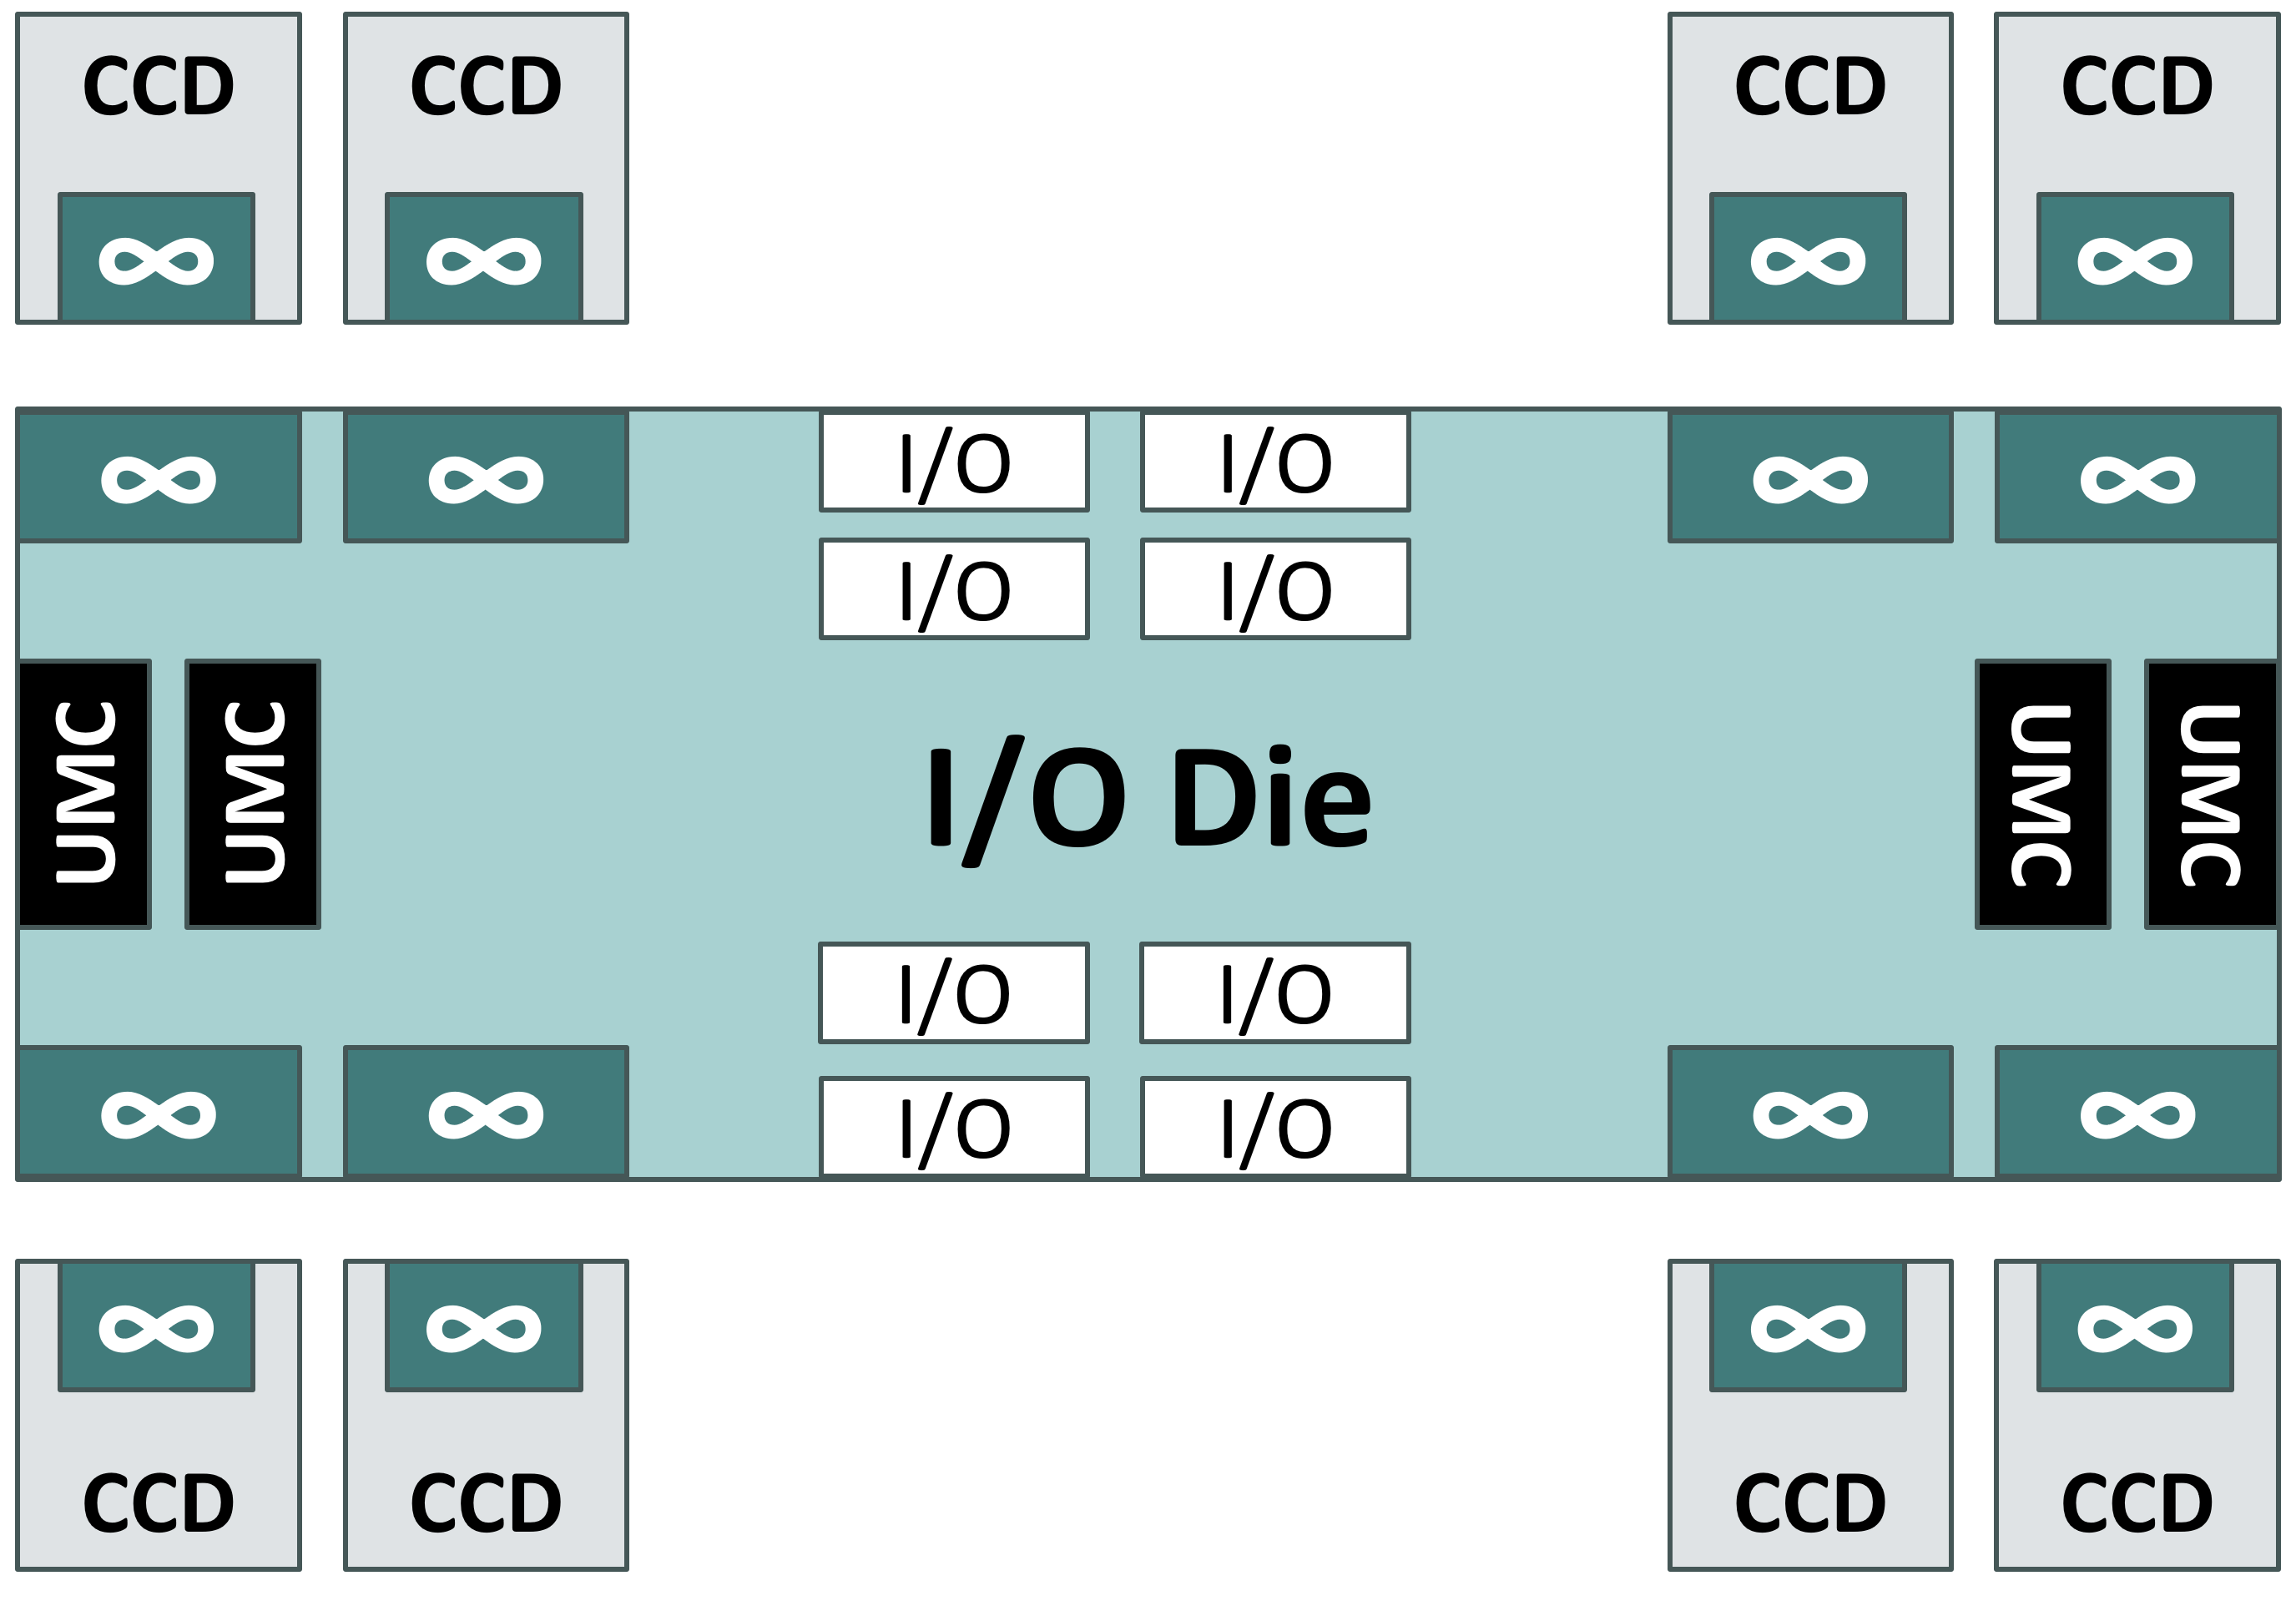
\includegraphics[width=\columnwidth]{figures/background/amd_arch/processor.png}
    \caption{AMD EPYC Zen 3 Architecture - CPU}
    \label{fig:amd-cpu}
\end{figure}


\Cref{fig:amd-cpu} shows a high-level overview of the architecture of the AMD EPYC Zen 3 processors.
The figure shows the following components:
\textbf{1) I/O:} The component that handles the input-output from the peripheral devices. This is where the PCIe communication happens.
\textbf{2) UMC:} The Unified Memory Controller is the controller that communicates with the DRAM.
\textbf{3) CCD:} The Core Complex Dies are where the cores (execution units) and caches reside.
\textbf{4) Infinity Fabric ($\infty$):} The interconnect that connects all of the components within the AMD CPU.

\subsubsection{CPU Pipelines}
\label{subsubsec:cpu-pipelines-bg}

Modern CPUs rely on executing multiple instructions simultaneously to maximise performance.
To achieve this, the CPUs have a multi-stage pipeline with the following stages: 1) Fetch, 2) Decode, 3) Schedule and Execute and 4) Retire.
We provide a simplified view of the pipeline in the CPU cores of the AMD EPYC Zen 3 processors in \Cref{fig:amd-core} and a brief description of each of the stages below:\\
\textbf{Fetch: } This stage fetches the next macro-op from the cache or the memory. 
However, the next macro-op to be fetched may not be deterministic, given the program may contain branches. 
In such cases, this stage also uses branch prediction to speculate on which instruction may be executed next and fetch that instruction.\\
\textbf{Decode: } This stage involved decoding the fetched macro-op into one or more micro-ops, which are then forwarded to the next stages.\\
\textbf{Schedule and Execute: } The scheduler(s) determine which instruction can be executed next based on the availability of the data that the instruction requires. 
This ensures that a long-running instruction (e.g., where the data is unavailable) does not stall all other independent instructions that can be executed.
As such, instructions here can be executed out of program order. 
Once the instruction has finished execution and the output of the instruction (if any) is available in the registers, the instruction is removed from the scheduler. 
\footnote{On AMD Zen 3 architecture, each scheduler has a capacity of 24 entries.}
As load and store are common but time-consuming instructions, this stage also consists of a load-store queue where pending load and store operations are held. \\
\textbf{Retire: } This stage ensures that instructions are retired in the program order so that the program can remain oblivious to the out-of-order execution that occurred in the previous stage.

\begin{figure}[!htb]
    \centering
    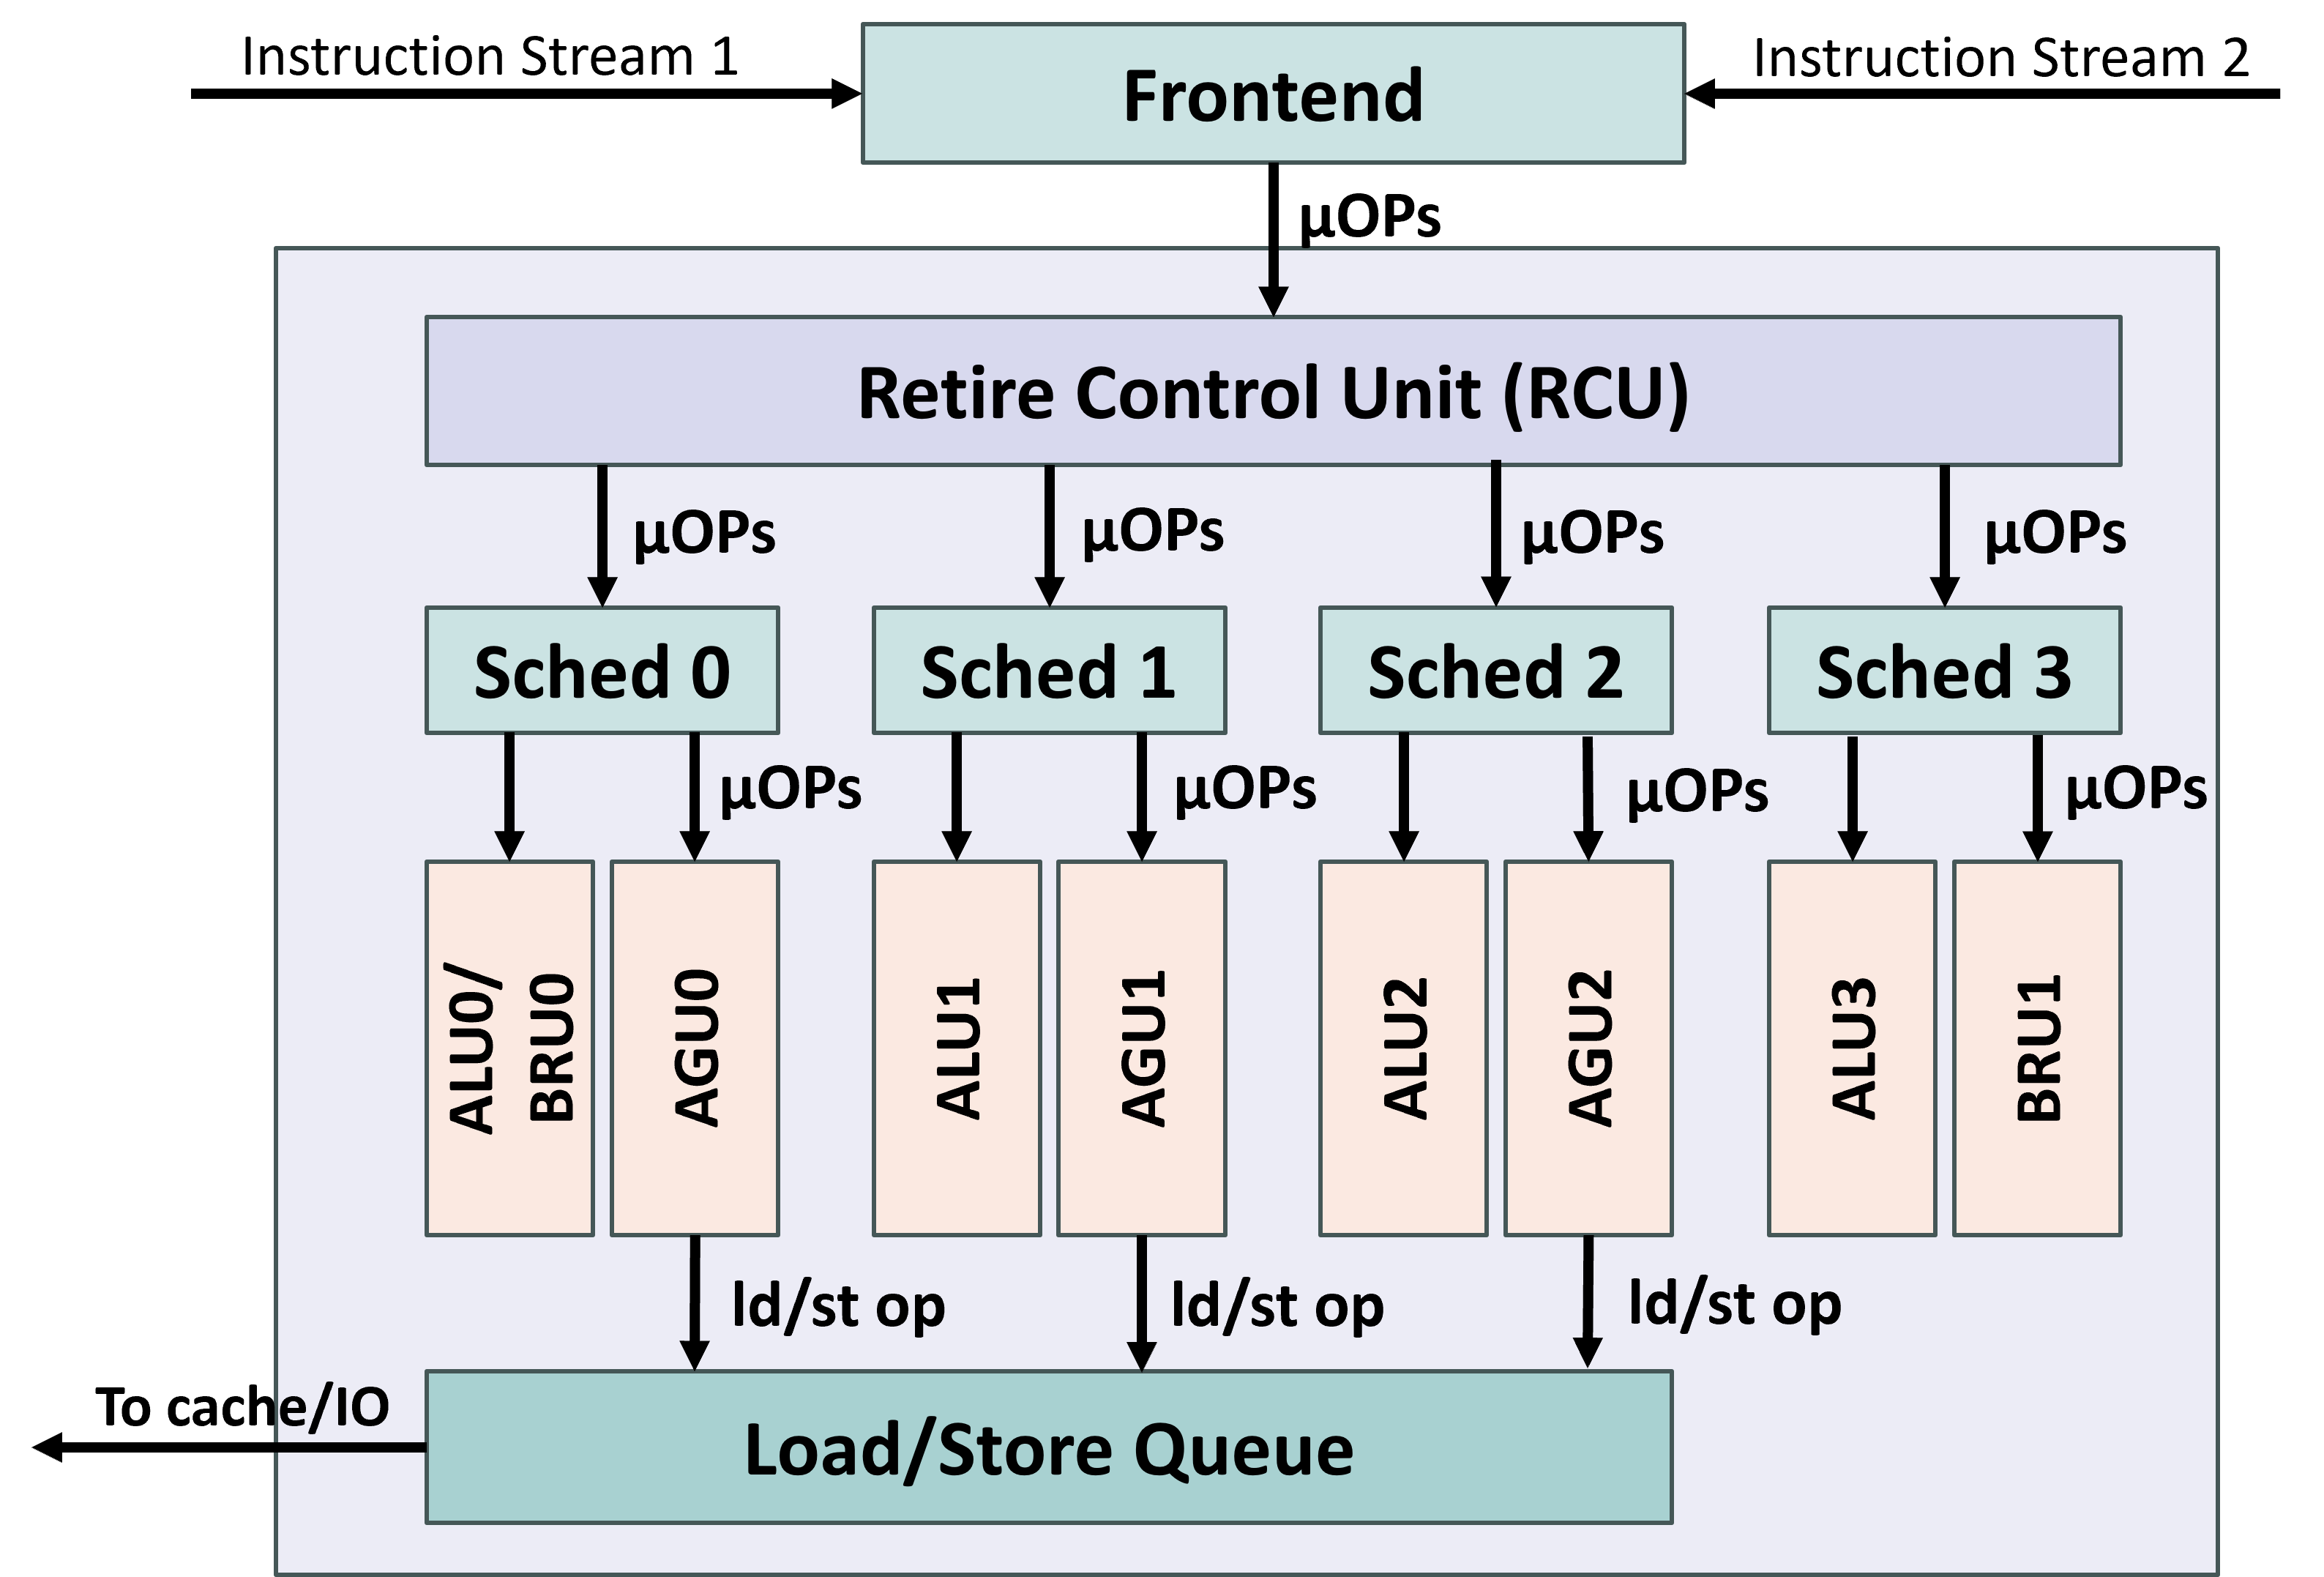
\includegraphics[width=\columnwidth]{figures/background/amd_arch/core.png}
    \caption{AMD EPYC Zen 3 Architecture - Core}
    \label{fig:amd-core}
\end{figure}

\subsubsection{PCIe transactions to/from CPU}

A program running on the CPU can transfer data to the PCIe device/endpoint in two major ways: 1) Memory operations via memory-mapped IO (MMIO) and 2) Direct memory access (DMA).
MMIO enables the CPU to map some memory region of the PCIe endpoint in the CPU's physical address space.
Any process with the proper permissions can then map this memory within the process and perform normal \textit{load} or \textit{store} operations on this memory.
However, this approach requires the execution units of the CPU to issue repeated \textit{load/store} instructions to copy data to the PCIe endpoint.
While this method is useful for reading or writing limited content, such as small configuration parameters, to the PCIe endpoints, it is inefficient for transferring a large amount of data.
To alleviate this, a lot of PCIe endpoints consist of a special hardware component called a DMA engine.
The DMA engine can copy large chunks of contiguous data without involving the execution units of the CPU.

For MMIO-based transactions, the load or store instructions go through the same instruction pipeline outlined in \Cref{fig:amd-core}. 
From the Load Store Queue, they end up in the I/O die outlined in \Cref{fig:amd-cpu} and go out the I/O block to the connected PCIe endpoint.
For DMA transactions (usually initiated by the PCIe endpoint), the transaction comes into the I/O block and, after some address and protocol translations, is sent out to the DRAM via the UMC.

\endinput


% \subsection{Threat Model}\label{subsec:interconnect-sc-threat-model}

\endinput
\chapter{NetShaper: A Differentially-Private Side Channel Mitigation System}

NetShaper \cite{sabzi2024netshaper} is both the name of the framework and the system that implements the framework to mitigate network side-channel attacks in internet applications.
We have provided a brief outline of the framework in \Cref{sec:netshaper-framework-bg}. 
Here, we describe the NetShaper system.

We first outline the requirements that the system should fulfil.
First, in any given window $W$, the system should be able to obtain the size of the payload in the buffering queue, with noise added to it. 
That is, the system should be able to complete the execution of $f_{DP}(S, t_{start}, t_{start} + W)$.
In the same window, the system should also be able to send out the payload, with padding, if necessary, such that the total data sent out, $b_{out}$, is equal to the noised size. 
However, it is sufficient to be able to queue $b_{out}$ bytes to be sent out, even if the actual transmission goes beyond the window $W$, as long as any delays were not caused by the payload coming in or already present in the buffering queue. 
The reason for this is the post-processing property of DP that we outlined in \Cref{subsec:dp-bg}.

Second, the payload and the padding should be indistinguishable to any observer observing the outbound packet stream.
Hence, the payload and padding should both be subject to the same congestion control, re-transmission, loss recovery, and other network behaviour.
In addition, the outbound transmission should provide the same or a higher level of reliability than the applications using this system expect.

Finally, the system should be modular so that modifications to any one sub-component do not require changes in the other components.
The system should also be portable and easily deployable, requiring none to minimal changes on the end hosts where the applications are running.
These goals ascertain that the system is easy to adopt and deploy and can easily be modified per the deployer's requirements.


% 1. Complete DP measurement within the window W
% 2. Data and Dummy should be indistinguishable
% 3. Should provide the same level of reliability the application expects
% 4. Should be modular for easy modification to sub-components
% 5. Should be portable and easily deployable, with minimal modifications of the end-hosts.

\section{Proxy Architecture}
\label{sec:proxy-arch}

\begin{figure}[!htb]
    \centering
    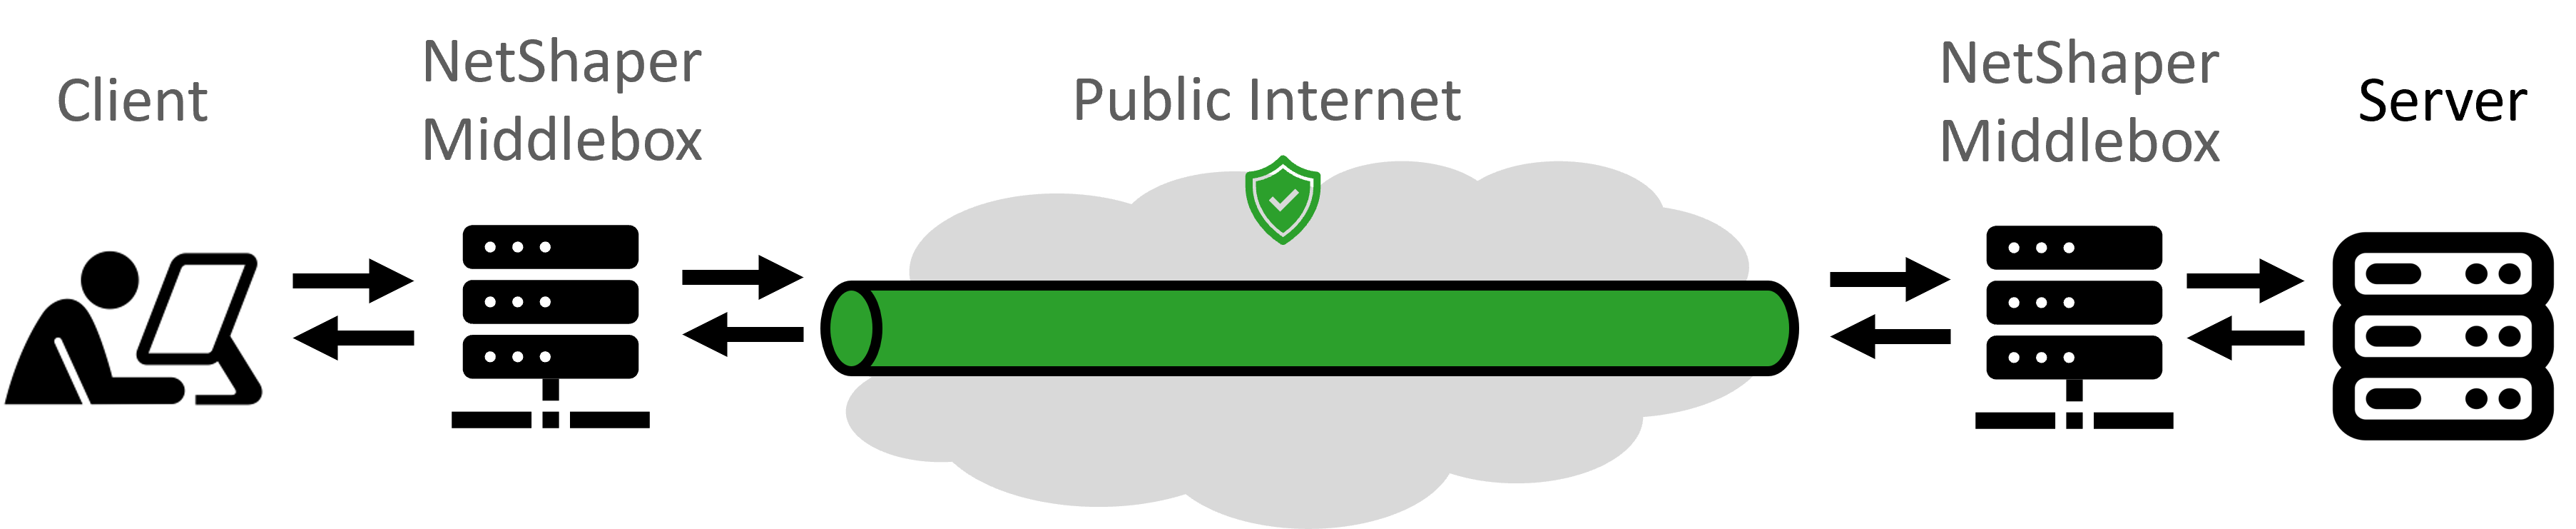
\includegraphics[width=\columnwidth]{figures/netshaper/netshaper-setup.png}
    \caption{NetShaper's Tunnel Setup}
    \label{fig:netshaper-setup}
\end{figure}

We designed NetShaper as a modular system that can be deployed using a pair of middleboxes, forming a forward and reverse proxy pair (see \Cref{fig:netshaper-setup}). 
Here, we describe in detail the architecture of the proxy setup and defer the discussion regarding the design of the middlebox to \Cref{sec:mb-design}. 

When using NetShaper, all clients communicate with the servers using three piecewise connections: 
(\textit{i}) between the client and the client-side middlebox, 
(\textit{ii}) between the client-side middlebox and the server-side middlebox, and
(\textit{iii}) between the server-side middlebox and the server.

For connection \textit{i} and \textit{iii}, NetShaper relies on standard TCP/UDP protocols. However, for connection \textit{ii} (i.e. to proxy the payload), NetShaper utilises QUIC. 
Using QUIC to proxy the payload avoids the TCP meltdown problem [??] that occurs when tunnelling TCP via TCP.
In addition, using QUIC also avoids the problem of an observer/attacker being able to distinguish between payload and padding that would occur when TCP was tunnelled via UDP (as the end host would retransmit payload, but the padding would not be retransmitted).

\paragraph{Setup.}
In order to be able to proxy end host traffic via NetShaper, the middleboxes need to be configured. 
The middleboxes first establish an encrypted QUIC connection between them, with user-specified reliability semantics.
Once the QUIC connection is established, NetShaper initialises three types of QUIC streams: Control, Data (Payload), and Dummy (Padding).
One \textit{control} stream is used to transmit messages regarding connection establishment or termination by the end host.
One \textit{dummy} stream is used for adding padding to the payload whenever necessary, based on the output of $f_{DP}$
\footnote{We avoid the use of PADDING frames in QUIC as they do not elicit acknowledgements and hence are distinguishable from the payload \cite{quic_rfc}.}.

\paragraph{Supporting multiple end hosts.}
As we discussed in \Cref{sec:quic-bg}, QUIC supports multiple streams in the same connection.
Using this, NetShaper can proxy the payload of multiple end hosts through a single QUIC connection between a pair of middleboxes.

While QUIC can support arbitrary initialisation and termination of streams, each stream has an associated header, which would increase the total transmission size.
For example, when transmitting two bytes in a single stream, the total transmission size would be $2 + S_{header}$.
However, when transmitting two streams of one byte each, the total transmission size would be $2 + 2*S_{header}$. 
An adversary may be able to distinguish between these two scenarios.
In order to avoid such a situation, NetShaper fixes and initialises a fixed number of streams per QUIC connection during the setup phase.
NetShaper assigns an unused stream to the client whenever a new client connects to the middlebox.
Similarly, NetShaper marks a stream as unused when an end host terminates the connection.

\endinput
\section{Middlebox Design}
\label{sec:mb-design}

While it is possible to apply NetShaper framework's approach at any network layer, we chose to develop the system as an L4 (Transport Layer) proxy.
This enables the system to be easily deployable, entirely in userspace and without requiring any superuser privileges. 
Developing NetShaper at L2 (Data Link Layer) or L3 (Network Layer) would require the deployer to either have the ability to modify the OS kernel or deploy some form of kernel bypass.

\begin{figure}[!htb]
    \centering
    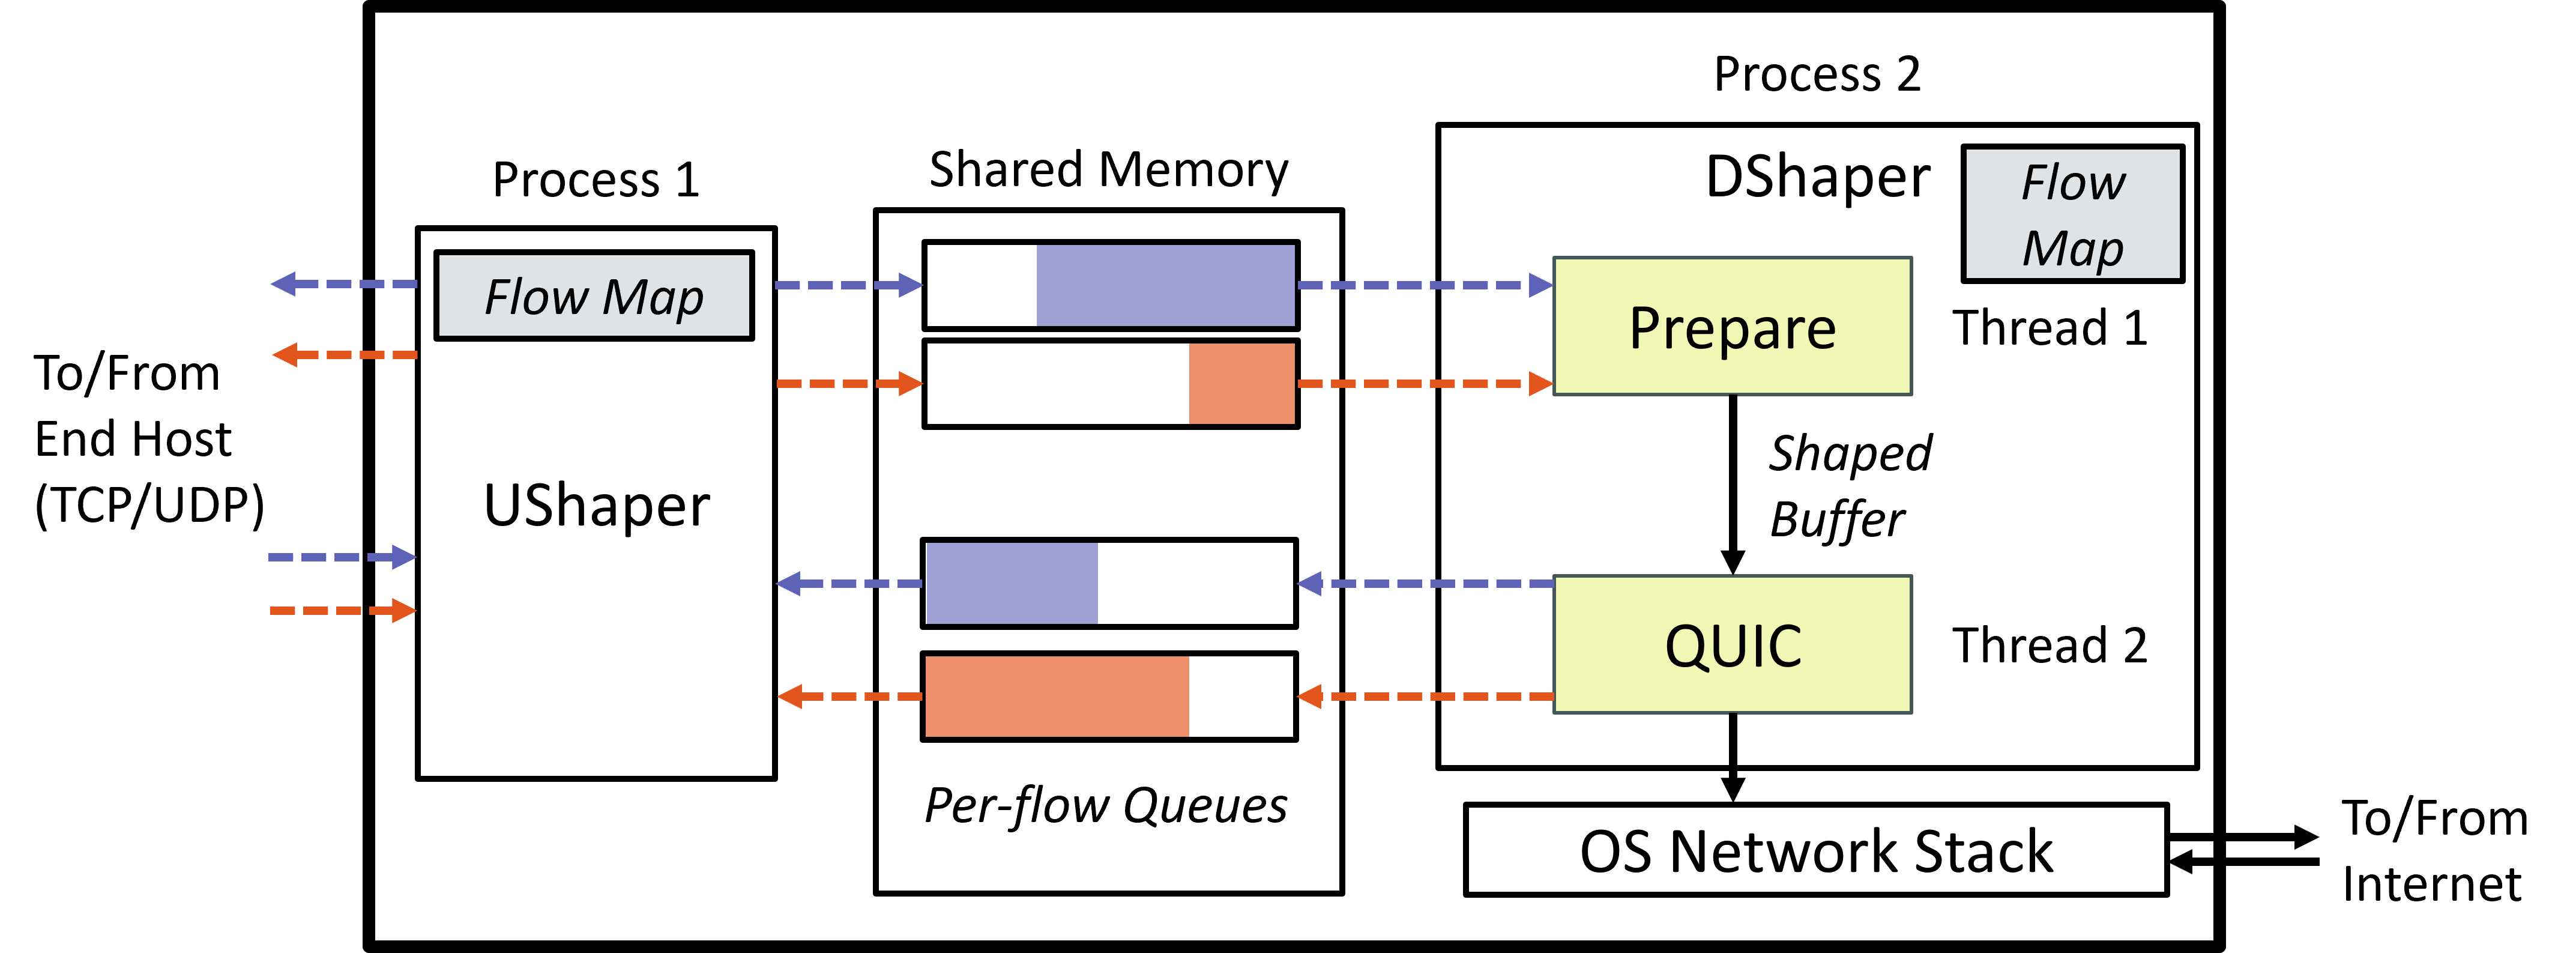
\includegraphics[width=\columnwidth]{figures/netshaper/middlebox-design.png}
    \caption{NetShaper Middlebox Design}
    \label{fig:middlebox-design}
\end{figure}

As outlined in \Cref{fig:middlebox-design}, NetShaper's middlebox consists of two main processes: UShaper and DShaper, and a shared memory between them.

\paragraph{UShaper.}
The \textit{UShaper} implements a client or a server to communicate with the end host.
It shares some Lamport Queues (LQs) [??] with DShaper.
It also consists of a flow map that maps a client with a corresponding pair of LQs.
\textit{UShaper} updates the flow map whenever a client establishes or terminates a connection.
In addition, it assigns an unused pair of LQs (one outbound and one inbound) to a new client and revokes that whenever the client terminates the connection.
The \textit{UShaper} receives outbound traffic from the end host and enqueues the payload in the assigned LQ.
Similarly, it dequeues inbound traffic from the inbound LQs and sends it to the corresponding end hosts.

\paragraph{DShaper.}
The \textit{DShaper} consists of two threads: \textit{Prepare} and \textit{QUIC worker}, and a flow map.
The flow map maps an LQ with a pre-initialised QUIC stream.
The \textit{Prepare} thread also measures the data available in the outbound LQs at the start of the window $W$.
It then adds noise to this available size based on the DP parameters.
Finally, it enqueues the payload and padding that needs to be transmitted.
The \textit{QUIC worker} transmits the enqueued data out to the network.
It also processes the received data, places it in the relevant LQ, and updates the flow map whenever a client initialises or terminates a connection.

In order to ensure that the operation of \textit{UShaper}, \textit{Prepare}, and \textit{QUIC worker} do not interfere with each other, we apply a few constraints in the implementation, and during the deployment of NetShaper.
First, all three components are required to be pinned on separate cores so that the execution time of one may not impact the others.
Second, in order to not leak the size of the payload due to the processing time of the enqueue operation done by the \textit{Prepare} thread, the \textit{Prepare} thread applies a lock for a fixed duration, during which the \textit{QUIC worker} can not transmit the data. 
We have outlined pseudo-code for both prepare and QUIC worker in \Cref{lst:prepare_and_worker}.
Finally, when receiving data, the \textit{QUIC worker} also enqueues the dummy bytes to a designated LQ so that the processing time remains consistent with the size of the data (see Figure ??).

\paragraph{Shared Memory.}
Both \textit{UShaper} and \textit{DShaper} have a shared memory between them.
This shared memory consists of three types of LQs: Control, Payload, Dummy
Similar to the stream types outlined in \Cref{sec:proxy-arch}, \textit{Control} LQ transmits the information about a connection establishment or termination by a client. 
\textit{Payload} LQ consists of the bytes received from the end host or to be sent to the end host.
\textit{Dummy} LQ consists of the dummy/padding bytes that are received.

\begin{minipage}{\textwidth}
\lstinputlisting[language=Python]{code/netshaper/prepare_and_worker.py}
\captionsetup{type=lstlisting}
\caption{Prepare and QUIC Worker Pseudo-code}
\label{lst:prepare_and_worker}
\end{minipage}

\endinput


\begin{figure}[!htb]
    \centering
    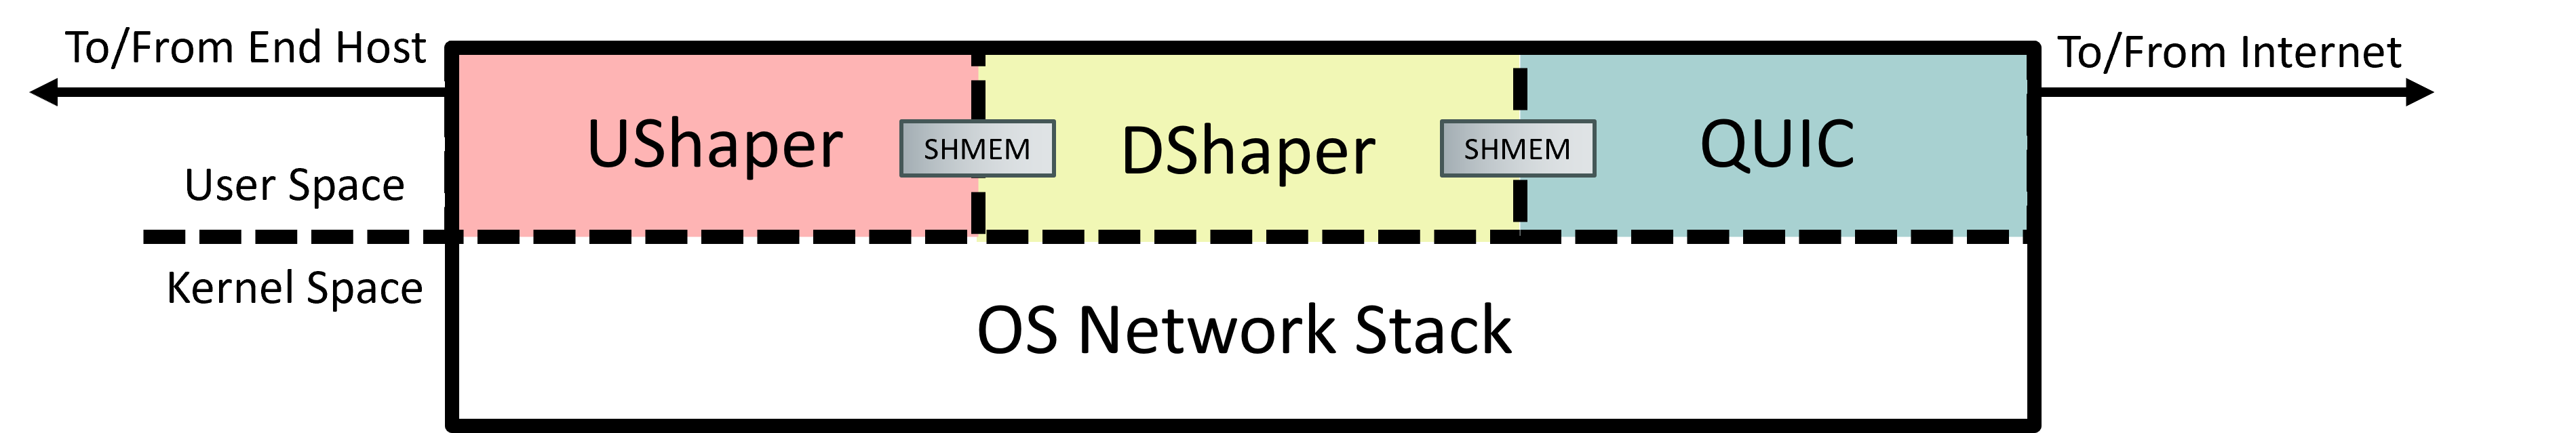
\includegraphics[width=\columnwidth]{figures/netshaper/middlebox-design-overview.png}
    \caption{Overview of NetShaper's Middlebox}
    \label{fig:middlebox-design-overview}
\end{figure}

\endinput

Should we add pseudo-codes for UShaper and DShaper?
\section{Performance}\label{sec:netshaper-performance}
\section{Limitations and Discussion}\label{sec:netshaper-discussion}

\endinput

\begin{singlespace}
\raggedright
\bibliographystyle{abbrvnat}
\bibliography{biblio}
\end{singlespace}

\end{document}
